
\documentclass{thesis}

\subtitle{Diplomarbeit}
\title{Algorithmen zur automatisierten Generalisierung durch Zusammenfassung von Linienzügen in OpenStreetMap\\ für konkrete Spezialfälle}
\author{Arne Johannessen}
\publishers{betreut durch\\ Prof. Dr. rer. nat. Detlef Günther-Diringer\\ und\\ Dipl.-Wi.-Ing. Frederik Ramm}
%\date{Arbeitsentwurf}
%\dedication{}

% je4
%\pdfinfo{
%  /Author (Name)
%  /Title (Titel der Diplomarbeit)
%  /Producer     (pdfeTex 3.14159-1.30.6-2.2)
%  /Keywords ()
%}
%\hypersetup{
%pdftitle=Titel der Diplomarbeit,
%pdfauthor=Name,
%pdfsubject={Diplomarbeit},
%pdfproducer={pdfeTex 3.14159-1.30.6-2.2},
%colorlinks=false,
%%pdfborder=0 0 0	% keine Box um die Links!
%}

\begin{document}

\maketitle

%\begin{abstract}
%\end{abstract}

\tableofcontents
% UTF-8

% single-chapter commands
\documentclass[../main/thesis.tex]{subfiles}
\begin{document}


\chapter{Einleitung \emph{[ausstehend]}}

\begin{itemize}
	\item erste, grobe Einführung ins Thema
	\item knapper Abriss des Kontextes der Fragestellung in Grundzügen (vgl. Themenblatt)
	\item was macht die Fragestellung interessant? (Motivation -- evtl. schon einzelne Anwendungsfälle umreißen)
	\item Gesamtüberblick der Arbeit einschließlich ihrer Ergebnisse, roter Faden als Orientierung für den Leser
	\item Eindruck an den Leser: warum soll er diese Arbeit weiterlesen oder welche Kapitel kann er überspringen
\end{itemize}

% auch Kontext _meiner_ Arbeit erklären -> Kooperation mit Geofabrik etc. -DGD
% Im weiteren Text der Arbeit können (und in gewissem Sinne _sollten_) Passagen aus dem Themenblatt 1:1 auftauchen, um den Bezug herzustellen. -DGD



% single-chapter commands
\end{document}

% UTF-8

% single-chapter commands
\documentclass{../thesis} \setcounter{chapter}{1} \begin{document}


\chapter{Analyse der Ausgangslage}

\section{OpenStreetMap: Alles für Alle}
Topographische Vermessungen führten ursprünglich nur zu relativ ungenauen Ergebnissen \cf[43]{Koh04}. Für die im 18.~und 19.~Jahrhundert erstmals durchgeführte systematische Landesaufnahme standen nur am Boden operierte Messinstrumente zur Verfügung. Bis in die zweite Hälfte des 20. Jahrhunderts waren der manuell horizontierte und abgelesene Theodolit und das Bandmaß die dabei primär eingesetzten Instrumente \cf[3–6]{WG06}. Deren Natur entsprechend ging dies mit einem immensen Aufwand an Arbeitskräften einher.

Die schiere Menge der eingesetzten Vermesser machte im Laufe der Zeit auch mit einfachen Instrumenten zufriedenstellende Ergebnisse möglich. In den letzten Jahrzehnten haben Photogrammetrie, Fernerkundung und satellitengestützte Ortsbestimmung das Vermessungswesen revolutioniert. Genauere Resultate ließen sich in kürzerer Zeit und so auch mit geringeren Kosten erreichen. \noref

% Ist die Kostendiskussion wirklich von Interesse? Eigentlich geht's ja nur um die ursprüngliche Motivation für OSM

Obgleich die Kosten geringer als zuvor sind, liegen sie nach wie vor in mehrstelliger Millionenhöhe allein für die amtlichen Geobasisdaten \cf[3]{lgm05}.
% [lgm05 3 (LG München, Beschl. vom 9. Nov. 2005, Az. 21 O 7402/02, 3; in: GRUR 2006, 225)]
In Europa \noref herrscht heutzutage \cf[119]{Fis01} die Auffassung vor, dass diese solcherart mit Steuergeldern erhobenen Daten der Allgemeinheit nicht kostfrei zur Weiternutzung zur Verfügung gestellt werden, sondern die \emph{konkreten} Nutzenden zusätzlich Lizenzgebühren zahlen sollen \noref. Diese Lizenzkosten schränken den Nutzen amtlicher Geodaten nicht nur für kommerzielle Zwecke \cf[336]{Böh07}, sondern auch für Privatleute \noref erheblich ein \noref.

% [Egg99 \noref]

Heute haben selbst billige GPS-Empfänger eine Genauigkeit, welche die mancher Vermessung des 19. Jahrhunderts übertreffen kann \cf[346][\?]{WG06}. Die „freie Weltkarte“ \eyecatcher{OpenStreetMap} (OSM) \cf[3]{RT09} macht sich dies zu Nutze, um mit Hilfe zehntausender Freiwilliger eine weltweite Datenbank mit Geobasisdaten aufzubauen und nachzuführen (Volunteered Geographic Information, VGI) \cf[147, 154]{NZ12}. Im Gegensatz zu vielen amtlichen Geobasisdaten dürfen OpenStreetMap-Daten lizenzkostenfrei verwendet werden, auch für kommerzielle Zwecke \cf[217, 221\f]{RT09}.

% ODBL? -> 3rd ed

% fühlt sich alles _viel_ zu lang an … was davon brauche ich wirklich als Überleitung zu Fragmentierung und Process?
% straff kürzen, unbekannte Begriffe a la KV-Pair einfach in Fußnote packen…

Der Name OpenStreetMap mag fehlleitend sein, denn es handelt sich dabei nicht um eine Straßenkarte, sondern vielmehr um eine Geodatenbank mit Inhalten nahezu beliebiger Themen. Bei der Gründung von OSM im Jahr 2004 wurde auf das Festlegen starrer Klassifizierungsschemata oder Kartierschlüssel verzichtet. Statt dessen kann jedes Element in der Datenbank mit einer beliebigen Anzahl Attribute – sogenannter \term{tags} – versehen werden, die jeweils aus einem Schlüssel und einem Wert bestehen \term{(key-value-pair)}. \cf[56]{RT09}

% ways / relationen / fragmentierung !!

Syntax und Semantik der einzelnen \term{tags} werden bei OpenStreetMap seit der Gründung fortlaufend von den Beitragenden diskutiert, gestützt auf bisherige Erfahrungen. Die Diskussion findet vornehmlich im Internet statt; Ergebnisse werden öffentlich dokumentiert und in Software wie z.~B. Renderern implementiert. Wer neue Inhalte erfasst, orientiert sich oft an den bisher in der Datenbank üblichen oder im Web dokumentierten Konventionen. \cf[48]{Top09} \cf[17\f, 59–66]{RT09}

Gegenüber einer vor der Erfassung detaillierten Ontologie \cf[\?]{GOS09} hat dieses System zur Folge, dass die zu OSM Beitragenden genau das erfassen, was sie persönlich interessiert und für wichtig halten. Jeder der Beitragenden entscheidet die Kriterien für die Erfassungsgeneralisierung für sich selbst. %Dies führt zu großen regionalen Unterschieden in Datendichte, -aktualität und -qualität.
% Regionalität ist nicht entscheidend für uns.

% Verweis auf Sch09 deckt schon vieles ab; Kne09 eher knapp, Beh11 noch knapper, Kla11 umständlich

Oft verfügen die OpenStreetMap-Daten über sehr hohen Detailreichtum. So könnten zum Beispiel für Teilstücke einer Straße \term{tags} für Tempolimits, Überholverbote, Fahrspurenanzahl, Oberflächenmaterial sowie -Qualität, Baujahr und mehr eingetragen worden sein. Veränderungen an diesen Attributen im Verlauf der Straße führen im OSM-Datenmodell zwangsläufig zu einer Fragmentierung in mehrere aufeinander folgende Linienabschnitte \term{(ways)}, jeweils mit unterschiedlichen \term{tags} \cf[57]{RT09}.

Baulich getrennte Fahrbahnen wie etwa Autobahnen bildet OpenStreetMap mittels zweier paralleler Einbahn-Linienzüge ab \cf[62]{RT09}. Dies ist eine in der Geoinformatik gängige Vorgehensweise \cf[2][\?]{Tho05}.

Sowohl die Fragmentierung als auch die parallelen Linienzüge führen zu Schwierigkeiten in der Weiterverarbeitung und Visualisierung \noref[Mig12 u. a.].
% Abbildungen:
% - Marker-Wucherung
% - stark unregelmäßige Plazierung von Namen \cf{Mig12}
% - Blitzer/Freistellung
% - Doppelnamen \cf{Mig12}
% o. ä.
Offensichtlich ist, dass eine Verkettung der Fragmente bzw. parallelen Linienzüge als Bestandteil des Datenmodells die Probleme wesentlich verkleinern, wenn nicht gar gänzlich lösen würde. Für eine hierarchisch orientierte Organisation wie etwa Vermessungsämter wäre eine solche Lösung naheliegend. Über \term{relations} ist dies auch in OpenStreetMap möglich \cf[57]{RT09}. Das oben beschriebene Fehlen interner Strukturen unter den zu OpenStreetMap Beitragenden (der \term{community}) macht es jedoch unmöglich, „mal eben“ die Regeln für die Erfassung und Kodierung der Geodaten zu ändern \cf{Sch09}.

Statt dessen müssen Änderungsvorschläge erst von der \term{community} akzeptiert und anschließend \emph{großräumig} und \emph{korrekt} in der Datenbank Anwendung finden. Die Erfahrung zeigt, dass dies ein langwieriger Prozess sein kann, der umso schwieriger wird, je geringer der unmittelbare Einfluss der Datenbank-Änderungen auf das in Karten sichtbare Ergebnis ist \noref.



%\biggap


\section{Kartenherstellung mit OpenStreetMap}

\begin{itemize}
	\item bisher im Wesentlichen nur automatische, (fast) ungeneralisierte Mercator-Tiles fürs Web
	\item Datenmenge, Maßstäbe, ständige Änderungen und Aktualisierungen etc.
	\begin{itemize}
		\item manuelle Generalisierung ist nicht zielführend außer für nicht nachzuführende Einzelanfertigungen
	\end{itemize}
	\item in der Praxis fast nur einfache semantische Modellgeneralisierung unmittelbar im Tile-Renderer, keine kartographische Generalisierung oder Folgekarten bzw. -datenbanken
	\begin{itemize}
		\item nahe beieinander liegende Punktsignaturen werden willkürlich selektiert, Linearsignaturen überdecken einander
	\end{itemize}
	\item insbesondere kaum Vereinfachung, Qualitätsumschlag, Zusammenfassung oder Verdrängung (jedoch einige lohnenswerte Ansätze, z. B. \cf{MWG12} oder Haltestellen-Relationen)
\end{itemize}

% Angesichts dessen wären automatisiert abgeleitete, generalisierte Datenbanken für kleinere Maßstäbe zur Weiterverwendung wünschenswert, existieren jedoch bisher nicht. Entsprechend sind auch die aus OSM-Daten hergestellten Karten in aller Regel nicht kartographisch generalisiert: Nahe beieinander liegende Objekte überdecken einander scheinbar wahllos, Mindestgrößen und notwendige Formvereinfachungen werden von den automatischen Renderern ignoriert.

% Erschwert wird die Generalisierung von OSM-Daten unter anderem durch den hohen Grad der Fragmentierung von Linienzügen. Das Verknüpfen solcher zusammengehörenden, einzelnen ways durch Relationen in der Datenbank ist technisch möglich, wird aber von den Mitwirkenden aus unterschiedlichen Gründen nur sehr selten durchgeführt. Eine automatisierte Generalisierung durch Formvereinfachung (zur Reduktion der node-Anzahl) bedingt daher, dass die zusammengehörenden ways  dabei  als solche identifiziert werden. Gleiches gilt für die Generalisierung durch Zusammenfassung oder Verdrängung parallel verlaufender Linienzüge, beispielsweise Straßen mit begleitendem Radweg oder mehrgleisigen Bahnstrecken.


\section{Automatisierte Linien-Generalisierung von OpenStreetMap-Daten}

\begin{itemize}
%	\item hier: ohne Flächen zu berücksichtigen, obwohl dort evtl. ähnliche Probleme auftreten könnten
% (ich glaube, ähnliche Probleme treten eigentlich nicht auf)
	
	\item Auswahl, Vergrößern und Betonen funktioniert zufriedenstellend
		\item einfache Screenshots aus osm.org als Beispiele
	
	\item Problem bei Verdrängung: der Konflikt (dass z. B. dicht beieinander liegende parallele Linienzüge parallel sind) muss erkannt werden, bevor verdrängt werden kann
		\item Skizze zur Erläuterung
	
	\item Problem bei Formvereinfachung: Fragmentierung sowie Erhalten der geometrischen Topologie
	\begin{itemize}
		\item Beispiel: Fluss außerhalb des (unabhängig gemappten) Flussbetts \cf[57]{Kla11}
			\item ebenso bei als Flächen gemappten Straßen oder bei landuse=railway
		\item Beispiel: ungleichmäßiger Abstand (teils sogar negativ, d. h. Überkreuzen) paralleler Fahrbahnen oder Gleise (Skizze oder Screenshot)
	\end{itemize}
	
	\item zumindest letzteres Beispiel ist lösbar durch vorhergehendes Zusammenfassen
	
	\item Problem bei Zusammenfassung: Linienzüge müssen (oft?) als zusammengehörig (z. B. parallel) erkannt werden, bevor zusammengefasst werden kann
	
	% Qualitätsumschlag? railway=rail -> landuse=railway ?
	
\end{itemize}


\section{Zielsetzung der Arbeit}

%\textbf{offener Punkt: Redundanz mit Themenblatt}

% Gedankensprung!
% (die Beispiele wiederholen sich => bessere Abgrenzung der Kapitel)

\begin{itemize}
	% „Algorithmen zur automatisierten Generalisierung durch Zusammenfassung von Linienzügen in OpenStreetMap“
	
	\item Erkennung als parallel ist bisher ein Problem
	
	\item Beispiel: Eisenbahnkarte mit untauglicher Darstellung von ein- und mehrgleisigen Strecken
		\item einfacher Screenshot von \url{http://www.itoworld.com/map/14?lon=8.06752&lat=49.22313&zoom=9}
	
	\item ein Problem nicht nur in kleinen, sondern auch in großen Maßstäben:
	
	\item Beispiel: unregelmäßige Lücken zwischen Autobahn-Richtungsfahrbahnen
		\item einfacher Screenshot von osm.org
	
	\item Formvereinfachungen von Parallelen ist ungelöst
	% ||
	\item Beispiele: untaugliche Formvereinfachungen (kurzer Verweis auf vorgenannte Probleme)
	% nur hier nennen...? -> bessere Kapitelabgrenzung!
	
	\item \eyecatcher{Ziel der Arbeit:} die automatisierte Generalisierung durch Zusammenfassung von Linienzügen
	
	\item Visionen:
	\begin{itemize}
		\item kartographische Generalisierung => besseres Kartenbild
			\item Zusammenfassung der Attribute derart, dass die Möglichkeit zur Darstellung der Gesamtwerte besteht (z. B. Railway-Tracks / lanes)
		\item Verringerung der Datenmenge => einfacheres Arbeiten mit Daten für große Gebiete, Vereinfachung der Weiternutzung
			(möglichst Zahlenbeispiele für Dateigröße, Featurezahl und/oder Laufzeiten anhand meiner Skripte für größere OSM-Datensätze nennen)
		\item Zusammenfassung kann theoretisch auch das Erstellen von MRDBs vereinfachen
	\end{itemize}
	
	\item \emph{nicht} Teil der Arbeit sind insbesondere:
	\begin{itemize}
		\item die Formvereinfachung selbst
		\item eine wie auch immer geartete Verdrängung (obgleich eine solche durch diese Arbeit vielleicht erleichtert werden könnte)
	\end{itemize}
\end{itemize}


\section[Diskussion existierender Ansätze]{Diskussion existierender Ansätze zur automatisierten Linien-Generalisierung}

\begin{itemize}

	% ! Puffer
	\item Puffer \cf[2–3]{OHSZ10}
% - für eine Darstellung von OSM-Daten als Teil eiens 3D-Modells werden Straßen "realistisch" verbreitert per Buffer in PostGIS
% - um Fragmente und Parallelen zu beseitigen, werden die so entstandenen Polygone nun vereinigt
% => Parallelen finden durch Buffer-Algorithmus und Polygonanalyse
% => Epsilon benötigt
% - Buffer orthogonal zur Linie würde reichen; die Endrundungen können wegfallen
% - löst Zusammenfassung nicht; evtl. inward offset (um wieviel?) oder eher -> Skeleton

	% ! Skeleton
	\item Skeleton \cf{LM96} \cf{Mig12} \cf[][\?]{All11}

% Mig12: <http://mike.teczno.com/notes/osm-us-terrain-layer/foreground.html>
% <http://twak.blogspot.de/2009/01/that-straight-skeleton-again.html>
% <http://www.ikg.uni-hannover.de/skalen/buendel/PDF/Skeleton.pdf>

	% ! OS MasterMap
	\item OS MasterMap
	% \cf{CM05}
	\cf{Tho05}

	% ! Strokes
	\item Strokes \cf{Tho06b} \cf{EM00}

	% ! graphbasiert
	\item graphbasiert \cf{JC04} \cf{MM99} \cf{HAS05} \cf{TR95} \cf{Kne09}

	% ! Relational Constraints
	\item Relational Constraints \cf{TBDJRG12}

	% ! Conflict Detection
	\item Conflict Detection \cf{KP98} \cf{Tho06a}

	% ! -> Christian Stern
	\item …

\end{itemize}

% + RoadMatcher 
% <http://wiki.openstreetmap.org/wiki/Roadmatcher>
% + http://sourceforge.net/projects/jump-pilot/files/OpenJUMP_plugins/More%20Plugins/Matching%20PlugIn/
% <http://sourceforge.net/projects/jump-pilot/files/OpenJUMP_plugins/More%20Plugins/Matching%20PlugIn/>

(jeweils einschließlich Anwendbarkeit auf die vorliegende Fragestellung, ggf. Vor- und Nachteilen, ggf. Bezug der darin verwendeten Fachsprache zur in dieser Arbeit verwendeten Terminologie)



\nocite{*}  % include works in bibliography that aren't cited anywhere in the document (for debugging)

% single-chapter commands
\listoffigures %\listoftables
\bibliographystyle{../myAMSalpha} \bibliography{../thesis}{}
\end{document}

\chapter{Spezifikation der zu untersuchenden Fälle}

\section[Vergleich verschiedener Problemfälle]{Vergleich verschiedener Problemfälle der automatisierten Linien-Generalisierung}

\begin{itemize}
	\item mehrgleisige Eisenbahnstrecken
	\item Richtungsfahrbahnen im Straßenraum mit baulicher Trennung
	\item parallele Fahrbahnen/Wege für unterschiedliche Verkehrsmittel/-arten
	\begin{itemize}
		\item z. B. zweibahnige Straße außerorts mit parallelem Zweirichtungsradweg
		\item z. B. Nebenfahrbahnen (Frontage Roads)
		\item z. B. straßenbündiger Bahnkörper (Straße mit Gleisen für Straßenbahn oder Street-Running)
		\item z. B. komplexe innerstädtische Straße mit mehreren parallelen getrennten Radwegen, Gehwegen, Richtungsfahrbahnen, Nebenfahrbahnen, besonderem Stadtbahn-Gleiskörper (mehrgleisig), Adressinterpolationen, PLZ-Grenze und unterirdischer Fernwärmeleitung
		\item z. B. Rampen für Anschlussstellen vom Typ SPUI (der "Fall Kriegsstraße") oder Diamant
	\end{itemize}
\end{itemize}

(Vergleich unter dem Gesichtspunkt der Eignung als "Spezialfall" für diese DA, vgl. Themenblatt)


\section{Auswahl der in dieser Arbeit zu behandelnden Spezialfälle}

\begin{itemize}
	\item Welcher konkrete Spezialfall wird in dieser Arbeit stellvertretend untersucht? Gibt es einen wesentlichen, die Auswahl entscheidenden Grund?
	\item Kann das Ergebnis dieser Arbeit auf andere Spezialfälle oder auf die Gesamtheit verallgemeinert werden? (kurze, grobe Abschätzung auf Basis der zuvor benannten Beispiele)
\end{itemize}


% UTF-8

% single-chapter commands
\documentclass[../main/thesis.tex]{subfiles}
\onlyinsubfile{\setcounter{chapter}{3}}  % single-chapter command
\begin{document}


\chapter{Algorithmen zur Generalisierung}

\section{Vorgehensweise}

...

% Erst über Generalisierung nachgedacht, da sie das schwierigerer Problem zu sein schien (in der Erwartung, die Identifikation ließe sich evtl. "nebenbei" lösen).
% Die Generalisierung ist auf den allerersten Blick ein einfaches geometrisches Problem, das keiner ausgefeilten Algorithmen a la 2.5 bedarf. Erst mal probiert, ob es sich so lösen lässt. Später festgestellt (-> Implementierung?), dass es in der Tat nicht so schrecklich schwierig war, jedoch die Entscheidung, was zusammengehört und was nicht, im Allgemeinen Fall schwieriger als erwartet war (ein Problem, das allerdings wohl auch für die Lösungen aus 2.5 bestanden hätte, womöglich gar in verstärktem Ausmaß).

% damals sehr früh (noch vor Anmeldung) den Algorithmus in groben Zügen aufgestellt und implementiert
% Vorgehen war im Prinzip, das Problem graphisch/geometrisch anzugehen und auf Papier zu lösen, dann in Code zu übertragen
% anschließend nur noch (sehr umfangreiche) Verbessserungen vorgenommen, insbesondere zur Flexibilisierung (individuellere Analyse, unterschiedliche Testdaten, Spezialfälle)
% zeitaufwändig: Alg. implementieren; insb.: Probleme im Workflow lösen (z. B. I/O), OOP, die Details des Alg. so hinbekommen, dass er halbwegs "rund" läuft, Probleme wie bei Kreuzungen
% habe versucht, ein wenig Test-Driven Development zu lernen, was mir schwer fiel, weil ich ständig die Struktur änderte
% erst versucht, rein geometrisch zu arbeiten, dann festgestellt (mit Jochen), dass bei Autobahnen etc Tags idR passen und die Sache erleichtern

% an dieser Stelle außerdem big picture: wie hängen die folgenden teile zusammen?
% -> lt. Themenblatt soll das Analyseergebnis auch separat von der Generalisierung zu verwenden sein!
% d.h. die Main-Klasse / Fassade sollte gar nicht hier beschrieben werden, das ist ein Implementierungsdetail (unter Kap. 5 zu beschrieben, wozu aber Kap. 5 wohl etwas umorganisiert werden müsste)
% anstatt des Analyser-Outputs ist tatsächlich bisher der CorrelationGraph das Analyseergebnis, jedoch noch unvollständig (man bräuchte noch eine Art Metrik, dass z. B. ab 80% parallelen Segmenten zwei Ways als parallel gelten; evtl. auch einen Append-Schritt, denn zur (verlangten) Identifikation paralleler Linienzüge müssten diese erst mal aus den Ways erzeugt werden, falls die Ways nicht ausreichen)

% im CLI sieht's im Moment in etwa so aus:
% 1. create OsmDataset (als InputDataset-Instanz, via ShapeReader)
% 2. Combiner.run
% 3. output
% also eigentlich nichts, was algorithmisch einer besonderen Beschreibung bedarf

% an dieser Stelle außerdem __Überleitung__: was kann man aus 2.5 für lehren/erkenntnisse ziehen? irgendwas anwendbares dabei? wenn ja, warum nicht?


%\section{Beschreibung der Algorithmen}

Im Folgenden werden die gefundenen Algorithmen zunächst in allgemeinen Begriffen beschrieben, wobei der Fokus auf ihrem Zusammenwirken und ihren Abhängigkeiten voneinander liegt.
Im Anschluss daran folgt ihre formale Beschreibung.

% erst Grundprinzip / -idee / -ansatz beschreiben, dann Edge Cases

\section{Grundprinzip}

Um das Zusammenfassen paralleler Linienzüge vorzubereiten, werden alle \term{nodes} des einen Linienzugs jeweils einem gegenüberliegenden \term{node} auf dem parallelen Linienzug zugeordnet.
Die Verbindung der Mittelpunkte zwischen den so einander zugeordneten \term{nodes} ergibt direkt den zusammengefassten Linienzug als Ergebnis der Generalisierung (Abbildung~\ref{fig:general-approach}).

Dieses Vorgehen vermeidet, dass die in Abschnitt~\ref{osm-fragmentation} besprochene häufige ungleichmäßige Fragmentierung von \osm-Linienzügen in mehrere \term{ways} einen Einfluss auf den Generalisierungsvorgang hat.
Aufgrund der nicht immer gleichen Anzahl und Verteilung der \term{nodes} kommt es vor, dass ein \term{node} des einen Linienzugs mehreren \term{nodes} des anderen Linienzugs zugeordnet wird, was jedoch unproblematisch ist.

\begin{figure}[ht]
  \begin{minipage}[t]{.5\linewidth}
    \centering
    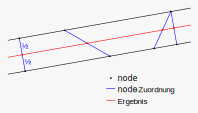
\includegraphics[width=\ScaleIfNeeded]{../chapter4/general-approach}
    \caption{general-approach}\label{fig:general-approach}
  \end{minipage}%
  \begin{minipage}[t]{.5\linewidth}
    \centering
    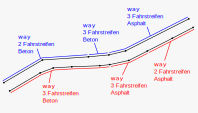
\includegraphics[width=\ScaleIfNeeded]{../chapter4/motorway-fragments}
    \caption{motorway-fragments}\label{fig:motorway-fragments}
  \end{minipage}
\end{figure}

Um zwei gegenüberliegende \term{nodes} einander zuordnen zu können, müssen zunächst die Linien, deren Teil sie sind, als zueinander parallel erkannt werden.
Auch hierbei ist die erwähnte ungleichmäßige Fragmentierung in bestimmten Fällen problematisch.
Beispielsweise müssten die einzelnen \term{ways} in Abbildung~\ref{fig:motorway-fragments}, aus denen die beiden dargestellten Parallelen bestehen, zunächst zu einem längeren Linienzug verknüpft werden, um einen Vergleich zu ermöglichen.
Dies entspräche dem in Abschnitt~\ref{os-mastermap} beschriebenen Ansatz von Thom, der damit zufriedenstellende Resultate erzielte, dabei jedoch die hohe Qualität seiner Ausgangsdaten betonte, welche bei wie für \osm{} von Freiwilligen erfassten Geodaten nicht vorausgesetzt werden kann.
% lässt sich diese aussage belegen?

Um diese Problematik zu umgehen, verwenden die in dieser Arbeit vorgestellten Algorithmen möglichst \emph{kurze} Liniensegmente anstelle möglichst \emph{langer} Linienzüge.
Die Verbindung zweier benachbarter \term{nodes} in einem \term{way} als kürzestmögliche lineare Einheit in den \osm-Ausgangsdaten (früher als \term{segment} bezeichnet \cf[57]{RT09}) ist allerdings für einen Vergleich nicht viel besser geeignet als der vollständige \term{way}%
% warum nicht? (wenig spezifisch formuliert)
, wie aus Abbildung~\ref{fig:motorway-fragments} ersichtlich ist.
Daher werden die \term{segments} für die Analyse auf Parallelität zunächst solange immer weiter unterteilt, bis schließlich ein einfacher geometrischer Vergleich möglich ist (Abbildung~\ref{fig:comparable-fragments}).

\begin{figure}[ht]
    \centering
    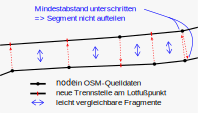
\includegraphics[width=\ScaleIfNeeded]{../chapter4/comparable-fragments}
    \caption{comparable-fragments}\label{fig:comparable-fragments}
\end{figure}



\section{Operationen}

Der zuvor beschriebene Lösungsansatz lässt sich vereinfacht als Sequenz von vier Operationen ausdrücken:\\
1. Segmente unterteilen\\
2. Analysieren\\
3. Punktezuordnung\\
4. Parallelen zusammenfassen\\

% Datenflussdiagramm

Die folgenden Abschnitte beschreiben jede dieser Operationen im Detail.

% Zur Vereinfachung Vorbedingungen der Eingabedaten: ...

% Definitionen: Ways haben Nodes; Segmente haben exakt zwei Nodes, welche mit folgender "Funktion zu erhalten sind; ...


\subsection{Segmente unterteilen}

In \osm-Daten sind seit Oktober~2007 Segmente (Verbindungen von exakt zwei \term{nodes}) nicht mehr als eigene Objekte enthalten \cf[57]{RT09}.
Anhand der aus der Datenquelle eingelesenen Menge aller \term{ways} $W$ wird daher zunächst durch \textproc{Segmentierung} die Menge aller Segmente $S$ ermittelt.

\begin{algorithm}[H]
\caption{Segmentierung}\label{alg:Segmentierung}
\begin{algorithmic}
\Function{Segmentierung}{$W$}%\Comment{$W$ ist die Menge aller \term{ways} der Datenquelle}
	\State $S \gets \varnothing$
	\ForAll{$w \textbf{ mit } w \in W $}
%		\State $N \gets$ alle \term{nodes} von $w$
%		\ForAll{$i \textbf{ mit } i \in \mathbb{N} : 0 < i < |N| $}\Comment{alle \term{nodes} außer dem ersten}
%			\State $n \gets$ \term{node} $i$ aus $N$
%			\State \textbf{füge} neues Segment ... \textbf{zu} $S$ \textbf{hinzu}
%		\ForAll{$n$ \textbf{mit} $n \in N \wedge \exists$ $m : m$ ist Vorgänger von $n$}
		\ForAll{$n$ \textbf{mit} $n \in w.nodes \wedge \exists$ $m : m$ ist Vorgänger von $n$ in $w$}
%			\State \textbf{füge} neues Segment $(m, n)$ \textbf{zu} $S$ \textbf{hinzu}
			\State $S \gets S \cup \{(m,n)\}$\Comment{neues Segment $(m, n)$ zu $S$ hinzufügen}
		\EndFor
	\EndFor
	\State \textbf{Ergebnis} $S$
\EndFunction
\end{algorithmic}
\end{algorithm}

Die Segmente $S$ werden anschließend durch \textproc{Splitten} derart in Fragmente aufgeteilt, dass ein geometrischer Vergleich leicht möglich wird (Abbildung~\ref{fig:comparable-fragments}).

\begin{algorithm}[H]
\caption{Splitten}\label{alg:Splitten}
$\textbf{Variable } gesplittet : Fragment \rightarrow bool$
\\$\textbf{Anfangswert } gesplittet(a) \stackrel{\text{\tiny def}}{=} nein$ $\forall$ $a$
\begin{algorithmic}
\Function{Splitten}{$S$}
	\State $B \gets S$\Comment{$B$ ist Liste zu splittender Segmente}
	\ForAll{$b := (n_1, n_2) \textbf{ mit } b \in B $}%\Comment{Segment $b = (n_1, n_2)$}
		\ForAll{$n \textbf{ mit } n \in \{n_1, n_2\} $}
			\ForAll{$t \textbf{ mit } t \in \textproc{NaheSegmente}(b) \wedge \neg$ $gesplittet(t) \wedge \exists$ $p_F : p_F = \textproc{Fußpunkt}(n, t)$}
				\State $\{f_1, f_2\} \gets \{(p_1, p_F), (p_F, p_2)\}$
%				\State $B \gets B \setminus \{t\} \cup \{f_1, f_2\}$
				\State $B \gets B \cup \{f_1, f_2\}$\Comment{Fragmente $f_1$ und $f_2$ rekursiv weiter aufteilen}
				\State $gesplittet(t) \gets ja$
			\EndFor
		\EndFor
	\EndFor
	\State \textbf{Ergebnis} $B$
\EndFunction
\end{algorithmic}
\end{algorithm}

% logisches Problem: Fragmente werden nicht dem R-Baum hinzugefügt, aber NaheSegmente liefert nur _Segmente_ aus dem R-Baum, folglich *keine* Rekursion (genauer: Rekursion nur von Fragmenten auf Segmente, nicht Fragmente auf Fragmente)

Für jedes Segment können dabei viele andere Segmente von vornherein als potenzielle Parallelen ausgeschlossen werden, beispielsweise solche, die zu weit entfernt und somit nicht \textproc{NaheSegmente} sind.
Nachdem die \osm-Eingangsdaten für die Generalisierung vollständig bekannt und somit statisch sind, bietet sich hierzu der Einsatz eines gepackten R-Baums an \cf[255-256]{RSV02}.

%2. Regionalisierung
%- ∀ Segmente : Liste der "nahen" anderen Segmente
%→ Spatial Index / Array (sortiert)

%\begin{algorithm}[H]
%\caption{Regionalisierung}\label{alg:Regionalisierung}
%$\textbf{Variable } naheSegmente : Segment \rightarrow \{Segmente\}$
%\\$\textbf{Anfangswert } naheSegmente(s) \stackrel{\text{\tiny def}}{=} \varnothing$ $\forall$ $s$
%\begin{algorithmic}
%\Procedure{Regionalisierung}{$S$}
%	\State neuer R-Baum $\mathcal{R}$
%	\ForAll{$s \textbf{ mit } s \in S $}
%		\State $s$ in $\mathcal{R}$ einfügen
%	\EndFor
%	\State $\mathcal{R}$ packen\Comment{R-Baum für Abfragen optimieren}
%	\ForAll{$s \textbf{ mit } s \in S $}
%		\State $N \gets$ Ergebnis der R-Baum-Abfrage für $s$
%		\State $naheSegmente(s) \gets N \setminus \{s\}$
%	\EndFor
%\EndProcedure
%\end{algorithmic}
%\end{algorithm}

%\begin{algorithm}[H]
%\caption{nahe Segmente}\label{alg:NaheSegmente}
%R-Baum $\mathcal{R}$
%\begin{algorithmic}
%\Function{NaheSegmente}{$s$}
%	\State $N \gets \{t : t \in \mathcal{R} \wedge H(s) \cap H(t) \neq \varnothing\}$\Comment{erweiterte Hülle $H$}
%	\State \textbf{Ergebnis} $N$
%\EndFunction
%\end{algorithmic}
%\end{algorithm}

\begin{algorithm}[H]
\caption{nahe Segmente}\label{alg:NaheSegmente}
\begin{algorithmic}
\Function{NaheSegmente}{$s$}
	\State Es sei $\mathcal{R}$ der bereits erzeugte und gepackte R-Baum. Ergebnis sei diejenige Teilmenge $N \subseteq \{r : r \in \mathcal{R}\}$ der im Baum enthaltenen Segmente $r$, deren Hülle $H(n) : n \in N$ die Hülle $H(s)$ des vorgegebenen Segments oder Fragments schneidet. Die Hüllfunktion $H$ liefere dabei die nach allen Seiten um $d/2$ vergrößerte rechteckige Hülle, wobei $d$ der festzulegende Höchstabstand sei, für den zwei Segmente oder Fragmente als „nahe“ gelten dürfen.
\EndFunction
\end{algorithmic}
\end{algorithm}

%3. Orientierungs-Ausschluss
%- ∀ Segmente : Liste der "nahen und geometrisch parallelen" Segmente

%, die weder zu weit entfernt sind noch deren Ausrichtung zu sehr abweicht.

%...

%4. Splitten ("re-entrant") in Fragmente
%Liste B aller `LinePart` als Basis (initial: alle `LineSegment`)
%- _∀ B : P₁, P₂_
%    - _∀ P_ als p
%        - _∀ `splitTargets()`_ : (_target noch nicht gesplittet_ -> next;)
%            - Fußpunkt PF für p auf target suchen
%            - falls nicht außerhalb target (✐) / falls ≠ target.P₁, target.P₂: *Split* target bei PF
%                - neue Fragmente f₁, f₂ mit P₁–PF und PF–P₂ erzeugen
%                - beide f₁, f₂ an Controller melden (für Basis-Iterator: hinten anhängen an Liste zu splittender Segmente)
%                - Basis und target als gesplittet / "fertig" markieren
%                - … mehr an Controller melden…?
%(`splitTargets()`: Liste der "nahen" anderen Segmente)

Das Aufteilen in Fragmente erfolgt jeweils am \textproc{Fußpunkt}~(Abbildung~\ref{fig:footpoint}).

\begin{algorithm}[H]
\caption{Fußpunkt}\label{alg:Fusspunkt}
\begin{algorithmic}
\Function{Fußpunkt}{$n,t$}
%	\State Es sei $l \bot t$ und $n \in l$. Dann sei $f \coloneq l \cap t$ bei $min(||f-t_1||, ||f-t_2||) > \varepsilon$ $\wedge$ $max(||f-t_1||, ||f-t_2||) < ||t||$, wobei $\varepsilon$ die festzulegende Mindestlänge eines Fragments sei.
	\State Ergebnis sei der Lotfußpunkt~$f$ des Punkts~$n$ auf der Geraden~$t$. Liegt~$f$ nicht zwischen den Punkten~$t_1, t_2$, welche $t$ definieren, oder liegt~$f$ näher an~$t_1$ oder~$t_2$ als die festzulegende Mindestlänge~$m$ eines Fragments, dann gibt es kein Ergebnis.
\EndFunction
\end{algorithmic}
\end{algorithm}

\begin{figure}[ht]
    \centering
    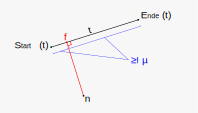
\includegraphics[width=\ScaleIfNeeded]{../chapter4/footpoint}
    \caption{footpoint}\label{fig:footpoint}
\end{figure}

\subsection{Analysieren}

Das Ergebnis der Operation „Segmente unterteilen“ eignet sich zur Analyse auf Parallelität.
Hierfür werden Geometrie und Attribute näher verglichen.

%5. Analyse der Fragmente
%∀ Fragmente:
%- Ähnlichkeitsmaß zu allen anderen in Frage kommenden Fragmenten bestimmen (⇐ `closeParallels`), sortieren
%- aussortieren über `Analyser`
%- ∀ verbleibenden anderen Fragmente: best match(es) L+R finden, falls vorhanden (teilen 2 Segmente einen Node, ist es kein Match! (sonst klappt die L/R-Punktfindung nicht richtig)
%- best match(es) für _Segmente_ eintragen in eine Liste (und zwar reziprok) (→ eigentlich unnötig??) (∀ Segmente: ∃ 2 Listen "paralleler" Segmente) L+R (|||)

...

\begin{algorithm}[H]
\caption{Analyse TBD}\label{alg:Analyse}
$\textbf{Variable } parallel : Segment \rightarrow (Seite links/rechts, Segmente)$
\\$\textbf{Anfangswert } parallel(a) \stackrel{\text{\tiny def}}{=} (b, \varnothing)$ $\forall$ $a,b$
\begin{algorithmic}
\Function{Analyse}{}
	\State \textbf{Ergebnis} $parallel$
\EndFunction
\end{algorithmic}
\end{algorithm}


%6. Links/Rechts filtern
%(Albaufstieg vs. Verteilerfahrbahnen)
%
%_defer_
%
%Basis: Vergleichsfaktor  
%z. B. _R_ ignorieren, falls Distanz zu _R_ *m*-fach Distanz zu _L_ ist (*m* ≈ 2,5)

...


\subsection{Punktezuordnung}

%7. Punktzuordnungen erzeugen (Vorstufe Generalisierung)
%
%- ∀ Segmente "S" : S hat Parallele und S noch nicht "fertig 7"
%    - ∀ Punkte (Start/End "T₁"), ∀ Seiten von S (L/R) "A"
%        - ∀ Parallelen von S "P" auf Seite A
%            - nahegelehensten Punkt finden "T₂"
%            - falls nichts gefunden (= keine Parallele auf dieser Seite), näcshtes A
%            - neue Punktzuordung: T₁ ↔︎ T₂
%    - S markieren als "fertig 7"
%
%_defer:_
%- ∀ Parallelen von S: Rekursion
%- alle Segmente/Zuordnungen für je ein ursprüngliches Segment als Teil eines "Blocks" markieren (könnte später evtl. Auffinden eines Anfangs zur Generalisierung erleichtern)

...

\begin{algorithm}[H]
\caption{Nodes Zuordnen}\label{alg:Zuordnen}
%$\textbf{Variable } fertig7 : Segment \rightarrow bool$
%\\$\textbf{Anfangswert } fertig7(a) \stackrel{\text{\tiny def}}{=} nein$ $\forall$ $a$
\begin{algorithmic}
\Function{NodesZuordnen}{$S,P$}
	\State $C \gets \varnothing$
	\ForAll{$s := (n_1, n_2) \textbf{ mit } s \in S$}% \wedge \neg$ $fertig7(t)$}
		\ForAll{$t_1 \textbf{ mit } t_1 \in \{n_1, n_2\} $}
			\ForAll{$p := (q_1, q_2) \textbf{ mit } p \in P(d,s)$ $\forall$ $d$}
				\State $t_2 \gets \begin{cases}q_1 & \text{für } ||t_1 - q_1|| \textless ||t_1 - q_2||\\q_2 & \text{sonst}\end{cases}$
				\State $C \gets C \cup (t_1, t_2)$\Comment{$t_2$ ist der $t_1$ am nächsten gelegene \term{node} von $p$}
			\EndFor
		\EndFor
%		\State $fertig7(s) \gets ja$
	\EndFor
	\State \textbf{Ergebnis} $C$
\EndFunction
\end{algorithmic}
\end{algorithm}


\subsection{Parallelen zusammenfassen}

%8. Generalisierung
%
%"trivialer Fall":
%1. zufällig Segment S wählen, Edge E (ES, ET) (Bedingung: Zähler E < 2)
%2. Richtung D zufällig wählen (-> S); {F,R}
%    1. gegenüberliegendes Segment T (für Start): dasjenige der beiden (<- trivialer Fall) Segment von ET, welches -- so gedreht, dass der Start-Node == ES ist -- in die gleiche Richtung zeigt wie S
%3. ∀ D :
%    1. wiederhole, solange ∃ E
%4. M-Punkt setzen
%    5. Segmente A,B von E in Richtung D: nächste Nodes N {X,Y} finden (falls ∄: N:= aktueller Node
%    6. ∀ N:
%        7. Edge F von N zurück zu E? (X->ET, Y->ES)
%           ∃: F ist nächstes E; Zähler E + 1, Zähler F + 1
%           ∄: continue 6, sonst: Edge F(X,Y)
%              ∃: F ist nächstes E
%      E=F <=> ∄: Zähler E + 1, continue 3

...


% hier noch ein weiterer Abschnitt 4.4 für den Gesamtüberblick


\section{alte Einteilung}

\subsection{Identifikation parallel verlaufender Linien-Fragmente}

Ansatz: Dieser Algorithmus eignet sich insgesamt weniger gut zur Identifikation als zur Generalisierung.
Die Identifikation erfolgt, indem festgestellt wird, ob eine Generalisierung notwendig ist oder nicht; falls sie notwendig ist, kann sie dann aber auch bereits recht billig durchgeführt werden.
Andererseits ist fraglich, welchen "praxistauglichen" Einsatz eine reine Identifikation ohne anschließende Generalisierung hätte.

Konzept (abstrakt):

1. nur Segmente betrachten (gerade Linienabschnitte, definiert durch zwei Punkte)

2. alle nahe beieinander liegenden Segmente auf Parallelität untersuchen

Die Segmente sind jedoch unterschiedlich lang und liegen teilweise etwas „verstreut“ im Raum, was die Untersuchung erschwert.
Deshalb werden die Segmente zunächst fragmentiert, indem benachbarte Segmente „geschickt“ weiter in kürzere Segmente unterteilt werden, so dass parallele Segmente immer ähnlich lang sind und einander gegenüberstehen.

Im Detail:

1. geometrische Indizierung (R-Tree) der Eingabedaten, um Suche nach nahen LineParts zu ermöglichen [regionalise]

2. $\forall$ LineParts: AbstractLinePart.splitCloseParallels, um gut vergleichbare Stücke zu erhalten (reentrant/rekursiv, d. h. neu erzeugte Fragmente werden bis zu einer Mindestgröße immer weiter aufgeteilt) [split]

3. $\forall$ LineParts: $\forall$ nahe Parallelen (laut Index): [analyse]

3.1 Vorprüfung (boolean)

3.2 Hauptprüfung (double)

3.3 best matches (links/rechts getrennt) speichern (keine Nachprüfung => falls das best match nicht passt, wird es trotzdem genommen, sofern nicht schon die vorprüfung die sache abgebrochen hat)
% offen: "realParallels"-Konzept
% geprüft werden die Fragmente, gespeichert werden die Segmente

% graphisch erklären, was genau passiert


\subsection{Generalisierung durch Zusammenfassung}

Konzept (in den allgemeinsten Begriffen):

1. Endpunkte der parallelen Segmente einander zuordnen

2. Der gesamte Graph wird "durchgehangelt", indem von einer CorrelationEdge ausgehend immer entlang der Segmente das nächste CorrelationEdge gefunden wird; diese Edges werden dann durch neu erzeugte Mittelpunkte miteinander verbunden.



% (Der CorrelationGraph ist ein Graph, in dem CorrelationEdges einander gegenüberliegende Knoten von parallelen Segmenten verbinden.)

% new GeneralisedLines
% - beliebige CorrelationEdge auswählen und von ihr ausgehend den angrenzenden Segmenten erst in die eine, dann die andere Richtung folgen, bis das Folgen nicht mehr eindeutig möglich ist (z. B. wegen einer Abzweigung)
% - dabei Mittelpunkte der CorrelationEdges jeweils einer neuen GeneralisedSection hinzufügen
% - Segmente, die nicht zusammengefasst wurden (weil keine Parallelen existieren), werden in Sections umgewandelt und ebenfalls den GeneralisedLines hinzugefügt, um einen homogenen Ergebnisdatensatz zu erhalten

...


\subsection{Verknüpfung von Linienfragmenten zu einem einzigen kontinuierlichen Linienzug}

...


% single-chapter commands
%\onlyinsubfile{\listoffigures} \onlyinsubfile{\listoftables}
%\onlyinsubfile{% global bibliography settings

\nocite{*}  % include works in bibliography that aren't cited anywhere in the document (for debugging)

\setbibpreamble{Die Literaturangaben sind alphabetisch nach den Nachnamen der Autoren sortiert. Bei mehreren Autoren wird nach dem ersten Autor sortiert.\par\bigskip\bigskip}

\bibliography{../references-papers,../references-manual}
%\bibliography{../references-manual}
}
\end{document}

% UTF-8

% single-chapter commands
\documentclass[../main/thesis.tex]{subfiles}
\onlyinsubfile{\setcounter{chapter}{4}}  % single-chapter command
\begin{document}


\chapter{Implementierung}

\section{Entwicklungsumgebung}

Zur Umsetzung der entwickelten Algorithmen in Software wurde die Plattform Java verwendet.
Die Wahl von Java erfolgte neben der Vertrautheit des Verfassers mit dem zugehörigen \term{framework} aufgrund zu erwartender Effizienzvorteile von kompiliertem Code gegenüber Skriptsprachen wie Perl.
% einer Empfehlung der Geofabrik folgend

Java als imperative Sprache erlaubt es nicht, Algorithmen mit dem gleichen Grad an Abstraktion zu beschreiben wie zuvor in Kapitel~\ref{ch:algorithm-parts} geschehen.
Dort konnten zugunsten einer vereinfachten
% jedoch präzisen, cf. EWD656
Beschreibung praktische Erwägungen wie der Bedarf an Rechenzeit und Speicherplatz teilweise hintenanstehen.
Bei der Implementierung in Java müssen hingegen sorgfältig solche Datenstrukturen gewählt werden, die eine effiziente Ausführung erlauben, und die Algorithmen soweit nötig entsprechend angepasst werden.
Das Ergebnis wird in Abschnitt~\ref{ch:data-structures} beschrieben.

Während der Entwicklung wurde versucht, so viel existierenden Code in Form von \term{frameworks} wiederzuverwenden wie möglich.
Diese Bestrebung verursachte Probleme, wie auch später in Abschnitt~\ref{ch:impl-difficulties} geschildert wird.
Bei der Entwicklung kamen zuletzt die folgenden Plattformen und \term{frameworks} zum Einsatz:

\begin{itemize}[nosep]
	\item Darwin 15.6 / Mac OS X 10.11.6
	\item Java™ Standard Edition JDK 8 Update 144\\ \url{http://www.oracle.com/technetwork/pt/java/javase/downloads/}
	\item Apache Ant 1.10.1 \quad \url{https://ant.apache.org/}
	\item args4j 2.33 \quad \url{http://args4j.kohsuke.org/}
	\item GeoTools 17.0 \quad \url{http://www.geotools.org/}
	% as of 2017-09-14, 17.1 is stable and includes one or two possibly useful bugfixes; 17.2 is not stable and can prolly be skipped
	\item TestNG 6.8 \quad \url{http://testng.org/}
	% http://web.archive.org/web/20121113133417/http://testng.org/testng-6.8.zip (all other releases appear to be corrupt; I'm probably doing something wrong)
	\item GDAL 2.2.1 \quad \url{http://www.gdal.org/}
\end{itemize}

Ursprünglich wurden ältere Softwareversionen verwendet.
Die nötigen Anpassungen an die hier genannten aktuellen Versionen waren gering, Kompatibilität mit den älteren Versionen ist jedoch gegenwärtig aufgrund von Änderungen in GeoTools nicht mehr gegeben.
Der Code ist dabei noch immer konform zum Syntax von Java 6. \cf{GJSB05}

Der folgende Abschnitt erläutert einige Überlegungen, die bei der Auswahl der \term{frameworks} relevant waren.



\section{Systemkonzept}

Für ein gut funktionierendes Gesamtpaket sind vor der Umsetzung von vorgegebenen Algorithmen in ausführbarem Code einige praktische Aspekte zu bedenken.

Zunächst stellt sich die Frage nach der Benutzerschnittstelle der Software.
Die gewählte Plattform Java bietet verschiedene Möglichkeiten, graphische Benutzeroberflächen (GUI) zu gestalten.
Denkbar wäre beispielsweise eine Integration in den weit verbreiteten \osm-Editor JOSM als \term{plug-in.}
Das Entwickeln und Debuggen einer GUI-Anwendung neigt jedoch dazu, zeitaufwändig zu sein.
Ohnehin würde es ein modularer Aufbau der Anwendung erlauben, zu einem späteren Zeitpunkt eine GUI zu ergänzen.
Aus diesen Gründen soll im Rahmen dieser Arbeit auf eine GUI zugunsten einer einfachen textbasierten Kommandozeilen-Schnittstelle (\term{command-line interface,} CLI) verzichtet werden.
Zum Parsen der CLI-Parameter bieten sich \term{frameworks} wie etwa args4j an.

Zur Verarbeitung beliebiger Geodaten müssen diese aus Datenspeichern eingelesen und wieder ausgegeben werden können.
Um Entwicklungszeit zu sparen, sollte hierfür nach Möglichkeit ein existierendes \term{framework} genutzt werden.
Zur Vermeidung einer zu engen Kopplung der Generalisierung an das gewählte \term{framework} ist es zu vermeiden, die Primitiven des \term{frameworks} intern weiterzubenutzen.
Stattdessen sollten eigene Datenstrukturen genutzt werden, um Modularität zu fördern.
Die dabei entstehenden Kosten in Form von Rechenzeit und Speicherverbrauch sind zu berücksichtigen.

Da die Algorithmen auf der euklidischen Ebene definiert sind (vgl. Abschnitt~\ref{ch:split-algorithm}), bietet es sich an, die Implementierung zunächst auf kartesische Koordinaten zu beschränken und zu verlangen, dass aus der \osm-Datenbank stammende Eingangsdaten nach Länge und Breite vor der Verarbeitung vom Benutzer in einem geeigneten Kartennetzentwurf abgebildet werden.
Grundsätzlich wären angesichts der hier durchzuführenden geometrischen Operationen winkeltreue Abbildungen wie etwa ein Mercator-Netz zu bevorzugen.
% Sny87, USGS PP 1395 p. 20
Aufgrund der üblicherweise geringen Abstände der Parallelen ist Winkeltreue jedoch kein strenges Kriterium.
% Wiederholung eines ähnlichen Gedanken in 4.3.1

Die in Abschnitt~\ref{ch:split-algorithm} gegebene Definition für \textproc{NaheSegmente} kann leicht mit Hilfe eines R-Baums umgesetzt werden.
Die \textproc{Hülle} ist dabei das minimal umgebende Rechteck eines Blatts im R-Baum.
Nachdem die \osm-Eingangsdaten vor der Generalisierung vollständig bekannt und somit statisch sind, bietet sich der Einsatz eines gepackten R-Baums an \cf[255-256]{RSV02}.
Ein solcher Baum wird von der JTS Topology Suite (JTS) angeboten, welche vom \term{framework} GeoTools als Implementierung des Geometriemodells verwendet wird.

GeoTools bietet außerdem Möglichkeiten zur Ein- und Ausgabe (\term{input/output,} I/O) von Geodaten in zahlreichen Formaten.
Zwar wird das native \osm-XML-Format ebensowenig unterstützt wie das neuere Protocol Buffer Binary Format (PBF).
Das verbreitete Format ESRI~Shapefile wird jedoch unterstützt.
Die Geofabrik stellt aktuelle OSM-Auszüge öffentlich als Shapefile bereit.
Alternativ lassen sich Shapefiles leicht mit gängiger Software wie etwa GDAL aus anderen Formaten erzeugen.
GDAL ermöglicht dabei auch den Zuschnitt auf ein abgegrenztes Untersuchungsgebiet, was sich für Testzwecke anbietet.

\onefigure{ht}{
	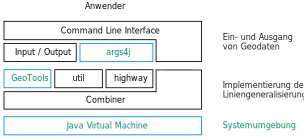
\includegraphics[width=\ScaleIfNeeded]{../chapter5/system-concept}
	\caption{Systemkonzept (schwarz: eigene Entwicklung, blau: benutztes \term{framework})}
	\label{fig:system-concept}
}

Zusammengesetzt ergibt sich aus den besprochenen Aspekten der in Abbildung~\ref{fig:system-concept} dargestellte Systemaufbau:
Dem Anwender steht eine Kommandozeilen-Schnittstelle (CLI) zur Verfügung, die ihrerseits das \term{framework} args4j zum Parsen der Parameter sowie selbst entwickelte Routinen zur Ein- und Ausgabe der Geodaten verwendet.
Die CLI steuert damit die eigentliche Liniengeneralisierung (hier als „Combiner“ bezeichnet), welche ihrerseits neben dem \term{framework} GeoTools noch einige selbst entwickelte Hilfsmodule verwendet, die nicht vom Combiner abhängig sind und deshalb als separates Softwarepaket dargestellt werden (mit „util“ bezeichnet).

% Noch mal Modularisierung; java Packages erwähnen/erklären? -> eher nein
% Ausgabe erfolgt nicht in OSM-Format. Hier erklären? -> eher später



\section{Datenstrukturen}
\label{ch:data-structures}

\begin{itemize}
	\item konzeptueller Überblick der entwickelten Software in dem Umfang, der für den Leser dieser Arbeit zum Verständnis notwendig ist
	\begin{itemize}
		\item z. B. Klassenstrukturen
		\item z. B. Interaktionswege
	\end{itemize}
	\item Bezug zu Kapitel 4 herstellen
\end{itemize}




\section{Schwierigkeiten bei der Umsetzung}
\label{ch:impl-difficulties}

\begin{itemize}
	\item Erläuterung wichtiger Designentscheidungen
	\item Unterschiede zu den entworfenen Algorithmen
	\item interessante konkrete Schwierigkeiten oder Erfolge bei der Implementierung aufzeigen
\end{itemize}


% single-chapter commands
%\onlyinsubfile{\listoffigures}
%\onlyinsubfile{\listoftables}
%\onlyinsubfile{% global bibliography settings

\nocite{*}  % include works in bibliography that aren't cited anywhere in the document (for debugging)

\setbibpreamble{Die Literaturangaben sind alphabetisch nach den Nachnamen der Autoren sortiert. Bei mehreren Autoren wird nach dem ersten Autor sortiert.\par\bigskip\bigskip}

\bibliography{../references-papers,../references-manual}
%\bibliography{../references-manual}
}
\end{document}

% UTF-8

% single-chapter commands
\documentclass[../main/thesis.tex]{subfiles}
\onlyinsubfile{\setcounter{chapter}{5}}  % single-chapter command
\begin{document}


\chapter{Ergebnisdiskussion}
% Beschreibung, was tatsächlich die Software ausspuckt, wo's hakt und wo ich noch gebastelt habe
% alles NUR im "Anwendungskontext", d.h. in Bezug auf die Ausgabe-Geodaten, nicht die Softwarequalität (das war in 5.4!)
% Schritt für Schritt Probleme sammeln und katalogisieren

Die in Kap. 4 und 5 entwickelte Software ist das Ergebnis dieser Arbeit. Hier diskutiert werden soll die Arbeitsweise dieser Software und die Qualität der von ihr ausgegebenen Geodaten in Bezug auf die Aufgabenstellung.

% möglichst auch Untersuchung der Anwendung des Algorithmus auf Straßen in unterschiedlichen Regionen der Welt



\section{Anwendung in einfachen Situationen}

Bei Anwendung der mit dieser Arbeit entwickelten Software auf Geodaten aus der \osm-Datenbank zeigt sich, dass die implementierten Algorithmen grundsätzlich funktionieren.

\onefigure{t}{
	\twofigures{H}{
		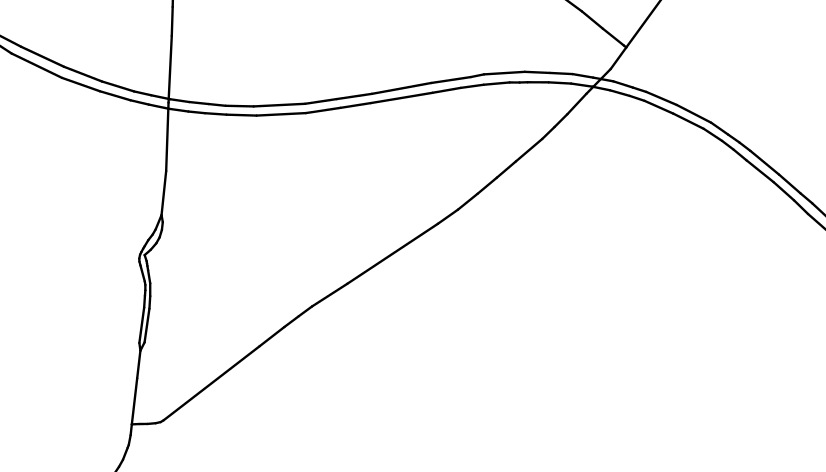
\includegraphics[width=\ScaleIfNeeded]{../chapter6/result-trivial-in}
	}{
		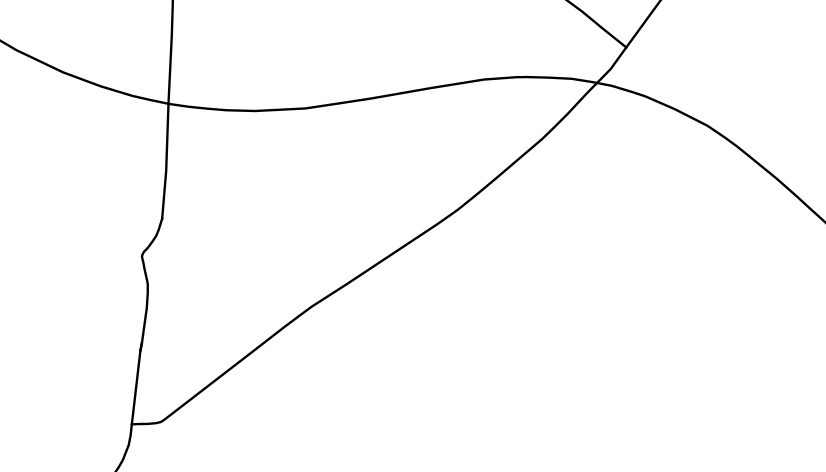
\includegraphics[width=\ScaleIfNeeded]{../chapter6/result-trivial-out}
	}
	% map extents (Google Mercator) 778753 6607040 780874 6608252; 0.2mm stroke
	\caption{Ergebnis der Software im einfachen Fall (links Eingangsdaten, rechts Generalisierungsergebnis; Autobahn L~124 bei Köln-Gremberg)}
	\label{fig:result-trivial}
}

In Abbildung~\ref{fig:result-trivial} sind links \osm-Linienzüge in der einfachen Situation einer Autobahn ohne Anschlussstellen nebst innerstädtischen Sammelstraßen zu sehen.
Durch Anwendung der Software ergibt sich das rechts dargestellte automatisiert zusammengefasste Ergebnis.
Anstelle der beiden Richtungsfahrbahnen der Autobahn gibt es nun nur noch eine gemeinsame Mittellinie.
Die Nähe zu nachgeordneten Straßen und deren planfreie Kreuzung mit der Autobahn stört die Generalisierung nicht.
Auch eine Strecke paralleler Fahrbahnen im nachgeordneten Netz wurde trotz eines scharfen Knicks erfolgreich als parallel erkannt und zusammengefasst.

Abbildung~\ref{fig:result-trivial-styled} zeigt beispielhaft, wie sich dieses Generalisierungsergebnis sinnvoll visualisieren ließe.
Die Software kennzeichnet die zusammengefassten Linienzüge als generalisiert.
Zusätzlich gibt die Software einzelne \term{tags} der \osm-Quelldaten mit aus.
Anhand dieser Attribute können leicht Regeln mit jeweils passenden Liniearsignaturen definiert werden.

\onefigure{t}{
	\twofigures{H}{
		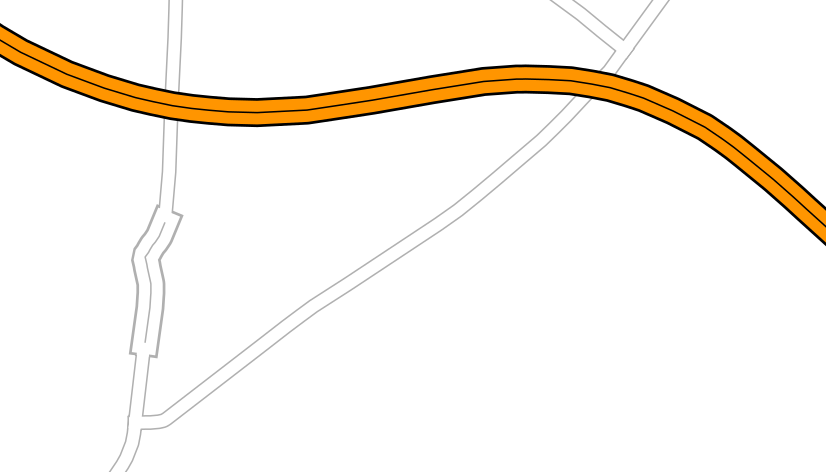
\includegraphics[width=\ScaleIfNeeded]{../chapter6/result-trivial-styled}
	}{
		\includegraphics[width=\ScaleIfNeeded]{../chapter6/result-trivial-rules}
	}
	\caption{Visualisierung des Generalisierungsergebnisses (links Kartendarstellung, rechts Screenshot der Zeichenregeln in QGIS)}
	\label{fig:result-trivial-styled}
}

\begin{itemize}
\item möglichst quantifizieren („bei Eingabedaten von xy km Autobahn gibt es z Problemsituationen“)
\item offen: Nicht-motorway/trunk sind schwieriger, da kleinere Kurvenradien. Funktioniert's hier? Wo nicht?
\item offen: Die \textproc{Distanz} zweier Straßen ist eines der wesentlichen Kriterien für die Erkennung als \textproc{Parallel}. Macht das Probleme, zB innerstädtisch vs. Autobahn?
\end{itemize}



\section{Attribute}

\begin{itemize}
\item (vorläufig) implementiertes Prinzip beschreiben
\item Auswirkungen: Beispiel, wo es nicht klappt?
\item möglichst quantifizieren
\end{itemize}



\section{Verhalten an Straßenkreuzungen}

\subsection{relocateGeneralisedNodes}

\begin{itemize}
\item tlws. gelöstes Problem: an Ende der Ausbaustrecke sowie innerstädtischer Kreuzung nodes von (nicht generalisierter) Querstraße so verschieben, dass es passt
\item offen: löst Problem nicht vollständig: funktioniert nicht (?), wenn Querstraße generalisiert ist?
\item (auch Problem im trivialen Fall, etwa in Heumar oder Kanalstraße/A57: Lücke in Topologie)
\item möglichst quantifizieren
\end{itemize}

% relocateGeneralisedNodes: "This is necessary because nodes are implemented as immutable by this project." -> Alternative: beide Nodes auf denselben Ort bewegen und dann als letzten Schritt Nodes am selben Ort erkennen und zusammenfassen (dann sollten aber sinnvollerweise auch die Node-IDs mitgeschleppt werden, sonst bringt das wenig, und die haben wir nicht, da wir OSM nicht direkt einlesen, sondern über die Geofabrik-Shapefiles gehen). Wichtig: *nur* wegen relocate() bekommt SourceNode die "edges" als Pointers!



\subsection{fehlende Kreuzungserkennung}

\begin{itemize}
\item fehlende Kreuzungserkennung
\item umfangreiche Problemdarstellung verschiedener Typen von Kreuzungen
\item möglichst quantifizieren
\end{itemize}



\section{Effizienz}

...



\section{Wiederholtes Ausführen für mehr als zwei Parallele}

...



\section{Anwendung auf andere Spezialfälle}

...



% single-chapter commands
%\onlyinsubfile{\listoffigures}
%\onlyinsubfile{\listoftables}
%\onlyinsubfile{% global bibliography settings

\nocite{*}  % include works in bibliography that aren't cited anywhere in the document (for debugging)

\setbibpreamble{Die Literaturangaben sind alphabetisch nach den Nachnamen der Autoren sortiert. Bei mehreren Autoren wird nach dem ersten Autor sortiert.\par\bigskip\bigskip}

\bibliography{../references-papers,../references-manual}
%\bibliography{../references-manual}
}
\end{document}

\chapter{Schlussfolgerung und Ausblick}

\section{Praktische Anwendbarkeit}

\begin{itemize}
	\item abschließende qualitative Gesamtbeurteilung der Arbeit auf Basis der Ergebnisuntersuchung in Bezug auf:
	\begin{itemize}
		\item Praxistauglichkeit
		\item Übertragbarkeit auf andere als die spezifizierten Spezialfälle
		\item Übertragbarkeit auf andere, ähnlich gelagerte, aber nicht identische Fragestellungen (z. B. Generalisierung durch Verdrängen)
		\item evtl. in Relation zu existierenden Lösungsansätzen (-> Analyse)
	\end{itemize}
\end{itemize}


\section{Ungelöste Problemfälle}

\begin{itemize}
	\item vorliegende Algorithmen und vorliegende Software
\end{itemize}


\section{Mögliche Ansätze zur Weiterentwicklung}

\begin{itemize}
	\item nächste Schritte
	\item neue Probleme
\end{itemize}


% Arbeit aus dem alten Standpunkt schreiben! Neuere Forschung etc. hier (und evtl. in Einleitung Kontext erklären) -DGD

% UTF-8

% single-chapter commands
\documentclass[../main/thesis.tex]{subfiles}
\onlyinsubfile{\setcounter{chapter}{7}}  % single-chapter command
\onlyinsubfile{\pagenumbering{roman}}
\begin{document}


\chapter{Zusammenfassung}
\label{ch:summary}

Das Projekt OpenStreetMap (OSM) hat das Ziel der Erstellung einer freien Geodatenbank auf Basis von \term{volunteered geographic information} (VGI).
Die weitere Verarbeitung und Visualisierung von \osm-Daten läuft in aller Regel voll automatisiert ab.
Sie wird erschwert durch den teilweise sehr hohen Detailreichtum, die daraus folgende Fragmentierung von Linienzügen sowie unvollständige Verknüpfungen zusammenhängender Geodaten wie etwa parallelen Richtungsfahrbahnen über Relationen im Datenmodell.

Eine kartographische Generalisierung von \osm-Daten findet bisher nur in geringstem Umfang statt.
Dies fällt unter anderem bei parallelen Richtungsfahrbahnen auf, deren Straßenachse in \osm\ nicht erfasst ist und bisher auch nicht in zufriedenstellender Weise automatisiert abgeleitet werden kann.
%Hier kommt es verbreitet zu unbefriedigenden Darstellungen wie etwa dem Unterschreiten kartographischer Mindestgrößen sowie Fehlern wie etwa dem Überkreuzen der beiden Richtungsfahrbahnen bei Formvereinfachung.
Ansätze zur automatisierten Zusammenfassung von Linienzügen existieren, sind jedoch auf \osm-Daten nicht gut anwendbar.
Insbesondere können sie Kreuzungssituationen oft nicht ohne besondere Attribute lösen.

Diese Arbeit stellt eine Methode zur Erkennung paralleler Linienzüge auf der Basis eines geometrischen Vergleichs kurzer Fragmente vor.
Linienzüge aus \osm\ werden so lange unterteilt, bis sich Stützpunkte auf Parallelen derart einander gegenüberliegen, dass eine Prüfung auf Parallelität leicht möglich ist.
Die anschließende Zusammenfassung der erkannten Parallelen ist dann einfach zu lösen.
Der Rechenaufwand der entwickelten Algorithmen wächst linear mit der Anzahl der Stützpunkte ($\mathcal{O}(n)$).
% eigentlich linear zur Anzahl der Segmente, aber deren Zahl ist proportional zur Anzahl der Stützpunkte, so dass dies keinen Unterschied macht

Zum Nachweis ihrer Funktionsfähigkeit und zum Test mit \term{real world}--Daten aus \osm\ erfolgte ihre ausführbare Implementierung.
Aufgrund einiger technischer Schwierigkeiten war dies aufwändiger als erwartet.
% was den Fokus ein Stück weit weg von der Kartographie hin zur Informatik verschob
Die mit Java entwickelte Software („Combiner“) hat erhebliches Optimierungspotenzial.

Wie sich zeigt, führt die mit dieser Arbeit entwickelte Methode in vielen Fällen zu einem guten Generalisierungsergebnis.
Jedoch leidet auch diese Methode an erheblichen Problemen in Kreuzungssituationen.
Aus Zeitgründen war es nicht möglich, eine praxistaugliche Lösung für diese Probleme zu finden.

% Attribute könnten hier noch erwähnt werden ... sie waren zwar bisher kein großer Teil der Arbeit, müssten es aber werden, wenn Praxistauglichkeit erreicht werden soll

Auch für andere, parallel entwickelte Methoden neueren Datums wird von ähnlichen Problemen in Kreuzungssituationen berichtet.
Eine offensichtliche Lösung mit allgemeiner Anwendbarkeit für das Problem der Zusammenfassung paralleler Linienzüge zeichnet sich derzeit nicht ab.
Es ist jedoch anzunehmen, dass eine zuverlässige automatisierte Kreuzungserkennung die Zusammenfassung zu einem leicht lösbaren Problem machen würde.
Diese Arbeit benennt dazu mehrere unterschiedliche mögliche Ansätze.



% unerwähnte wesentliche Punkte der einzelnen Unterkapitel:
% 2.5.2 u.a. Skelettlinien: (für DA zu) aufwändig, aber funktioniert zumindest halbwegs
% 2.5.4 u.a. Strokes: möglichst lange Linienzüge erzeugen, dann zusammenfassen [Thom]
% 2.5.5 u.a. Graphenanalyse: evtl. entfallende Parallelen durch Zusammenfassung von Kreuzungen
% 3.2 (Auswahl eines Spezialfalls: "baulich getrennte Richtungsfahrbahnen im Straßenraum")
% 4.1 (Diskussion der Tauglichkeit einiger Ansätze aus 2.5 für den gewählten Spezialfall)
% 4.1 Skelett nicht wegen Kreuzungsproblemen, Strokes nicht wegen fehlenden Attributen [Thom]
% 4.1 statt möglichst langer Linien (Strokes) auch gleichmäßig kurze Linien denkbar
% 5.3 Datenmodell der Bibliothek GeoTools hier schlecht geeignet
% 5.3 eigenes Datenmodell als Alternative, auf "möglichst kurze Fragmente" zugeschnitten
% 6.2 OSM-Datenqualität hinsichtlich Attributen problematisch
% 6.4 Performance zufriedenstellend, jedoch Speicherverbrauch offenbar optimierungsfähig
% 6.5 auch auf andere Spezialfälle anwendbar, aber derzeit mit erheblichen Einschränkungen



\chapter*{Summary}
\addcontentsline{toc}{chapter}{Summary}

The goal of the OpenStreetMap project (OSM) is the creation of a free spatial database using volunteered geographic information (VGI).
Further processing and visualisation of \osm\ data almost always takes place fully automated.
This is impeded by the in parts very high amount of detail, the resulting fragmentation of line strings as well as incomplete linkage of spatial data belonging together by means of relations in the data model.

So far, cartographic generalisation of \osm\ data only happens to the most limited extent.
Among other situations this is noticeable at dual carriageways, whose centreline is not included in \osm\ and cannot yet be automatically derived in a satisfactory manner.
Approaches for the automatic generalisation of line strings exist, but are not well suited for \osm\ data.
In particular they are often unable to find solutions for junctions without special attributes.

This thesis presents a method for the detection of parallel line strings on the basis of a geometric comparison.
Line strings from \osm\ are fragmented further until vertices on parallels exist opposite to each other such that verifying the parallelism is simple.
The subsequent merging of the detected parallels is then easy to solve.
The computational complexity of the developed algorithms grows linear with the number of vertices ($\mathcal{O}(n)$).

An executable implementation of the algorithms demonstrates their operability and allows for testing with real world data from \osm.
Due to some technical difficulties development was more time-consuming than expected.
The software (“Combiner”) has considerable potential for optimisation.

The approach developed in this thesis leads to a good generalisation result in many cases.
However, this approach has significant problems at junctions as well.
Developing a viable solution for these problems was not possible due to time constraints.

There are also reports of similar problems at junctions for other approaches that were developed in parallel to this thesis.
An obvious solution with general applicability for the problem of merging parallel line strings is not currently apparent.
It can however be expected that a reliable automated junction detection would turn the merging into a simple problem.
This thesis lists several distinct potential approaches to this end.



\end{document}


\listoffigures
\listoftables
% unified list: see KOMAscript 135

\nocite{*}  % include works in bibliography that aren't cited anywhere in the document (for debugging)
\setbibpreamble{Die Literaturangaben sind alphabetisch nach den Nachnamen der Autoren sortiert. Bei mehreren Autoren wird nach dem ersten Autor sortiert.\par\bigskip\bigskip}
\bibliographystyle{myAMSalpha}
\bibliography{thesis}{}

%\appendix
%\chapter{Glossar}
%\chapter{Abkürzungsverzeichnis}
%\chapter{Software-Dokumentation}

\end{document}
